\chapter{Results}
\label{chap:evaluation}

To evaluate the newly implemented functionality, a series of test cases are used. These test cases are created by directly manipulating the model's vector graphics using the \textit{Firefox Developer Tools}. Individual vertices can be manipulated directly within the browser by decoding a \textit{base64}-encoded string that represents the graphic into a readable format that describes the properties of the corresponding \textit{.svg} file. Adjustments to attributes such as \textit{fill} followed by re-encoding the data into \textit{base64} allows changing the appearance of the visualization. Similarly, vertex positions can be modified, or vertices can be removed entirely, by adjusting the relevant values within the developer tools.\\
All test cases are derived from the models shown in \autoref{fig:unaltered_layers} and are simulated with minimal deviations to ensure accuracy.

\section{Test Cases}
\label{sec:test_cases}
Because the Error indications differ based on the step of the pipeline the error was found in, the testcases are divided into three categories:
\begin{itemize}
    \item Testcases where the error can be indicated textually as well as visually highlighted inside the editor (see \autoref{tab:test_cases}).
    \item Testcases where the error can only be indicated via a textual error indication (see \autoref{tab:test_cases_text}).
    \item Testcases without any simulated errors to illustrate the pipeline's capability to deal with complex models (see \autoref{tab:functional_test_cases_no_errors}).
\end{itemize}
\autoref{tab:test_cases} shows the results of testcases where the error can be identified and visually highlighted inside the \acrshort{xgee} Editor, as well as indicated via the textual log. The first column in \autoref{tab:test_cases} provides a brief description of the simulated error and the used error model. The second column provides an image of the relevant portion of the screenshot with the error highlighted. If the error type is found to be \textit{Untokenized Pixels}, the highlighting color is purple, otherwise, the color is red. The third column provides the textual error indication alongside the step of the verification pipeline, where the error was detected. In some cases, for example when a device with multiple \acrshort{io}s is removed or too small to be detected, many error indications of the same type are generated. In this case, only a few of the error indications are shown in the table and further errors of the same type are indicated using `` $\lowvdots$\ ''.

\begin{figure}[htb]  \centering
    \begin{minipage}{0.4\textwidth}
        \centering
        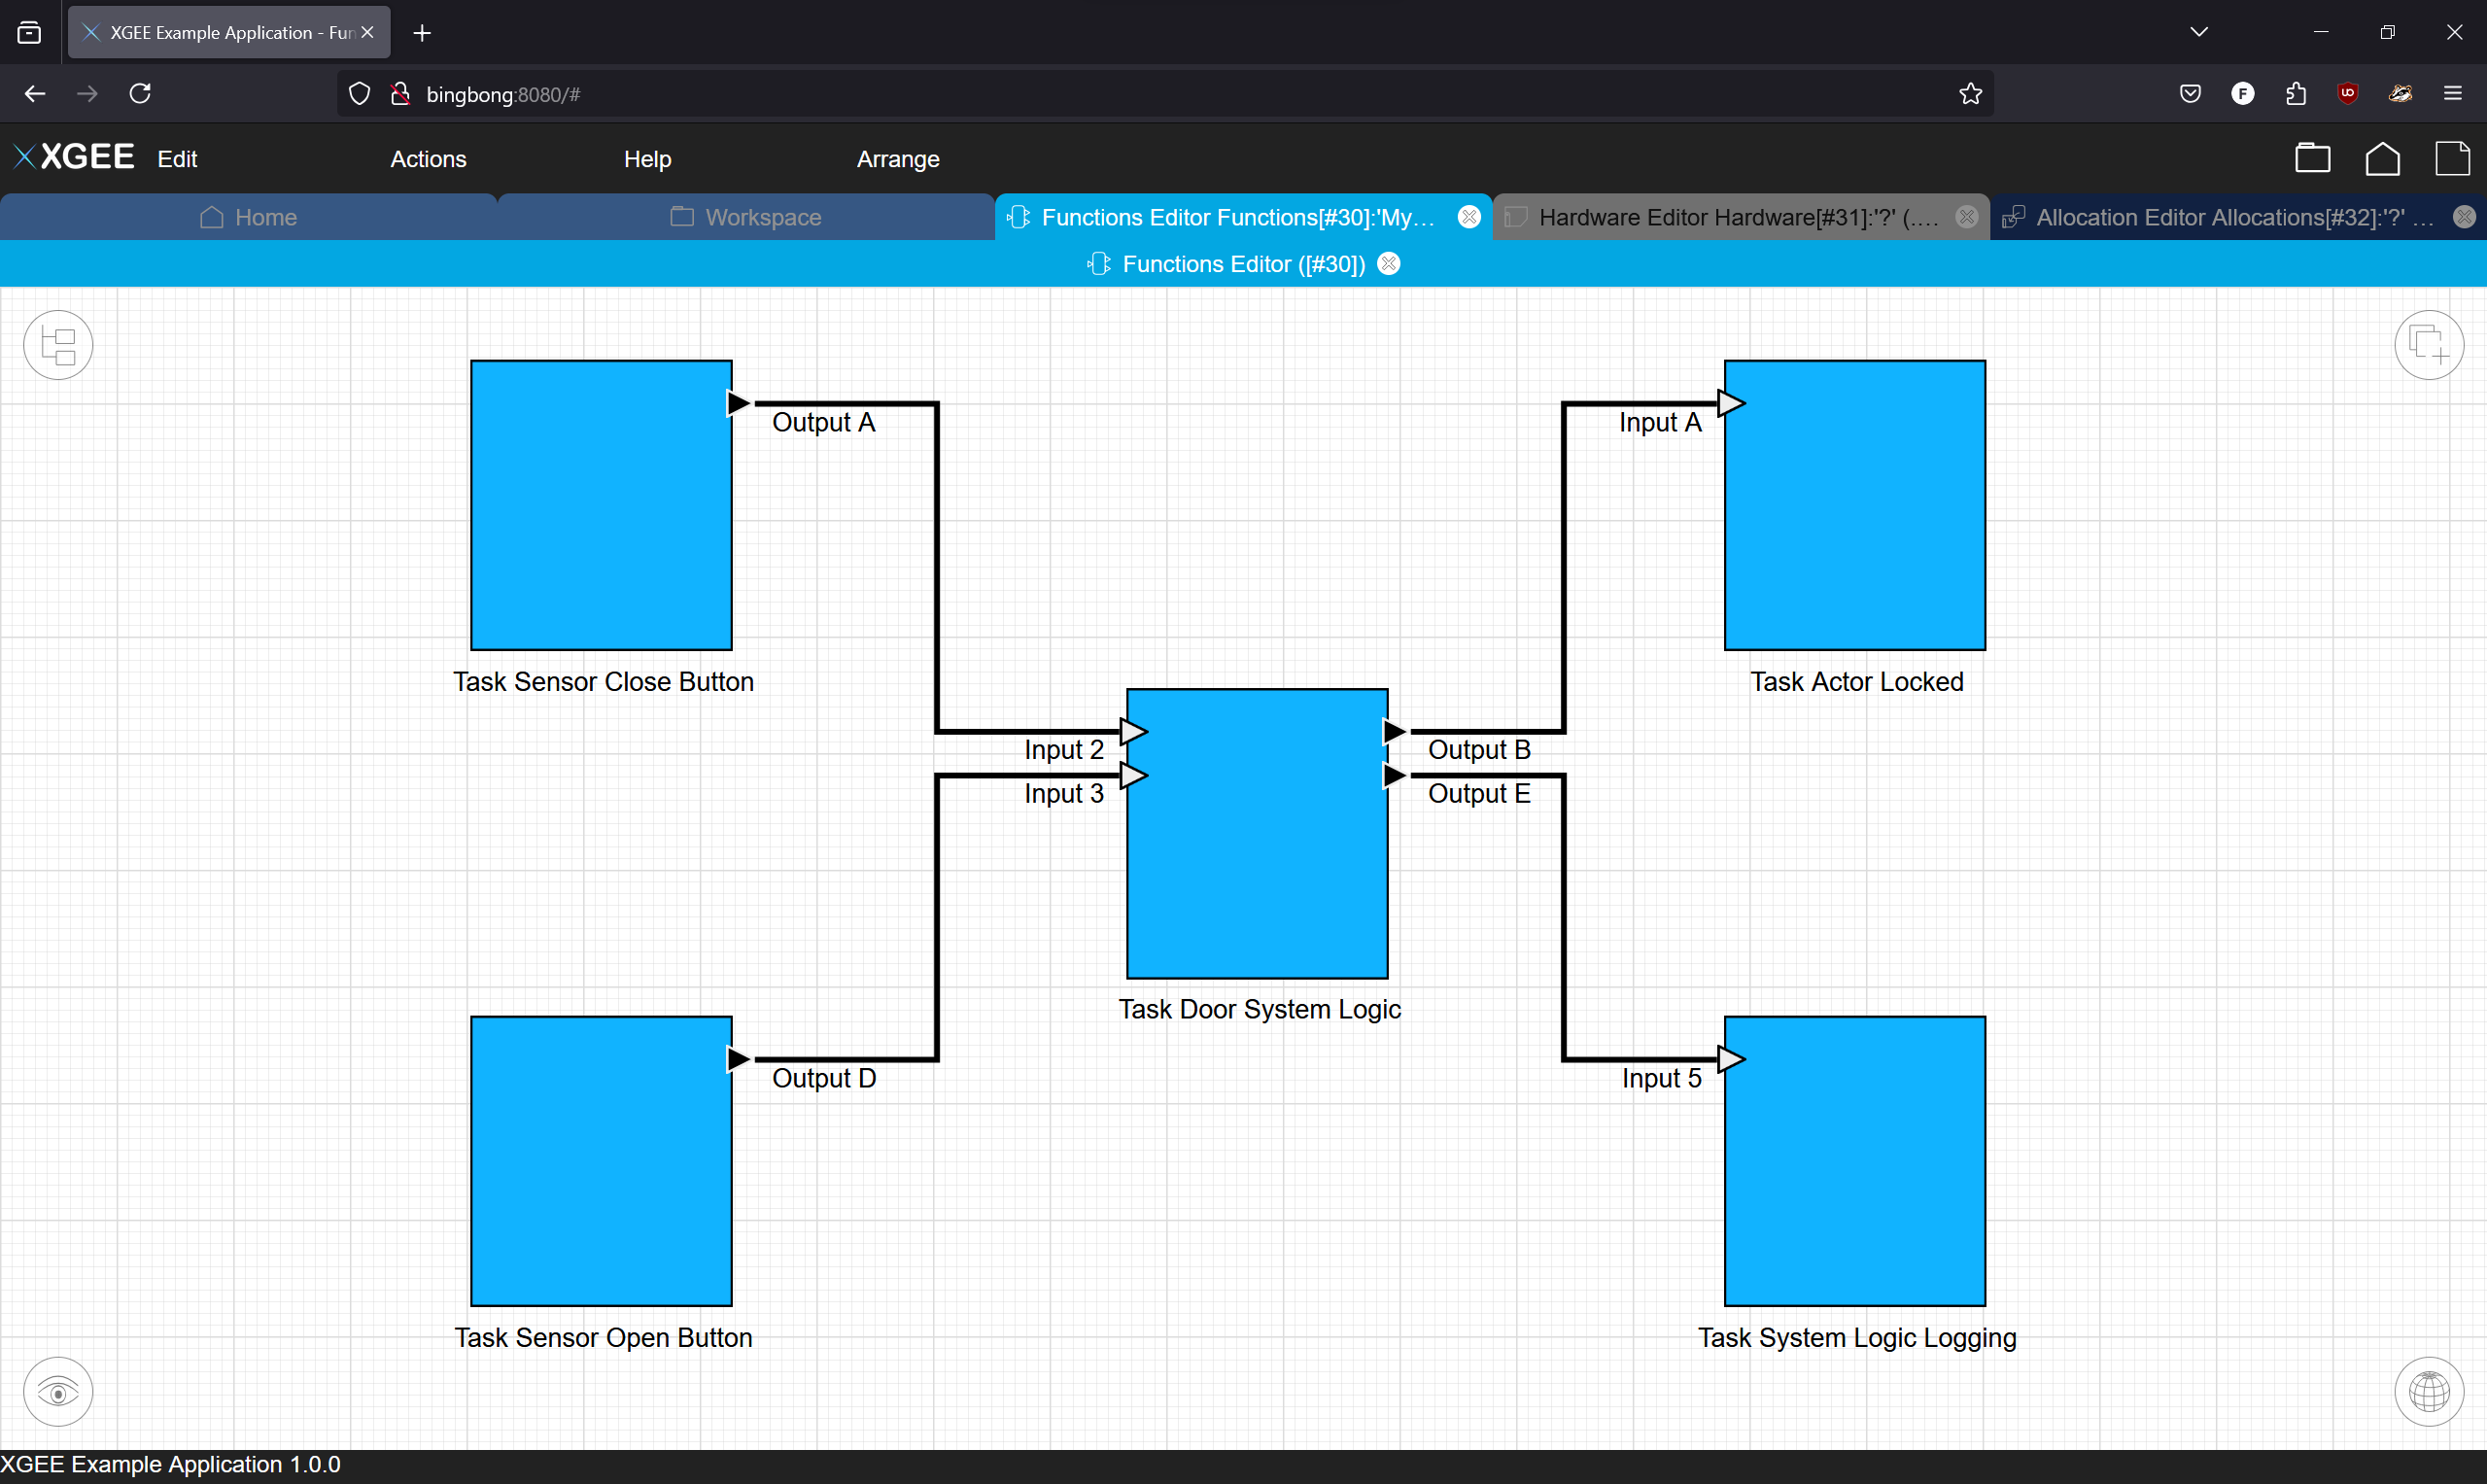
\includegraphics[width=\textwidth]{pictures/functions_unaltered.png}
        \label{fig:functions_unaltered}
    \end{minipage}
    \hfill
    \begin{minipage}{0.4\textwidth}
        \centering
        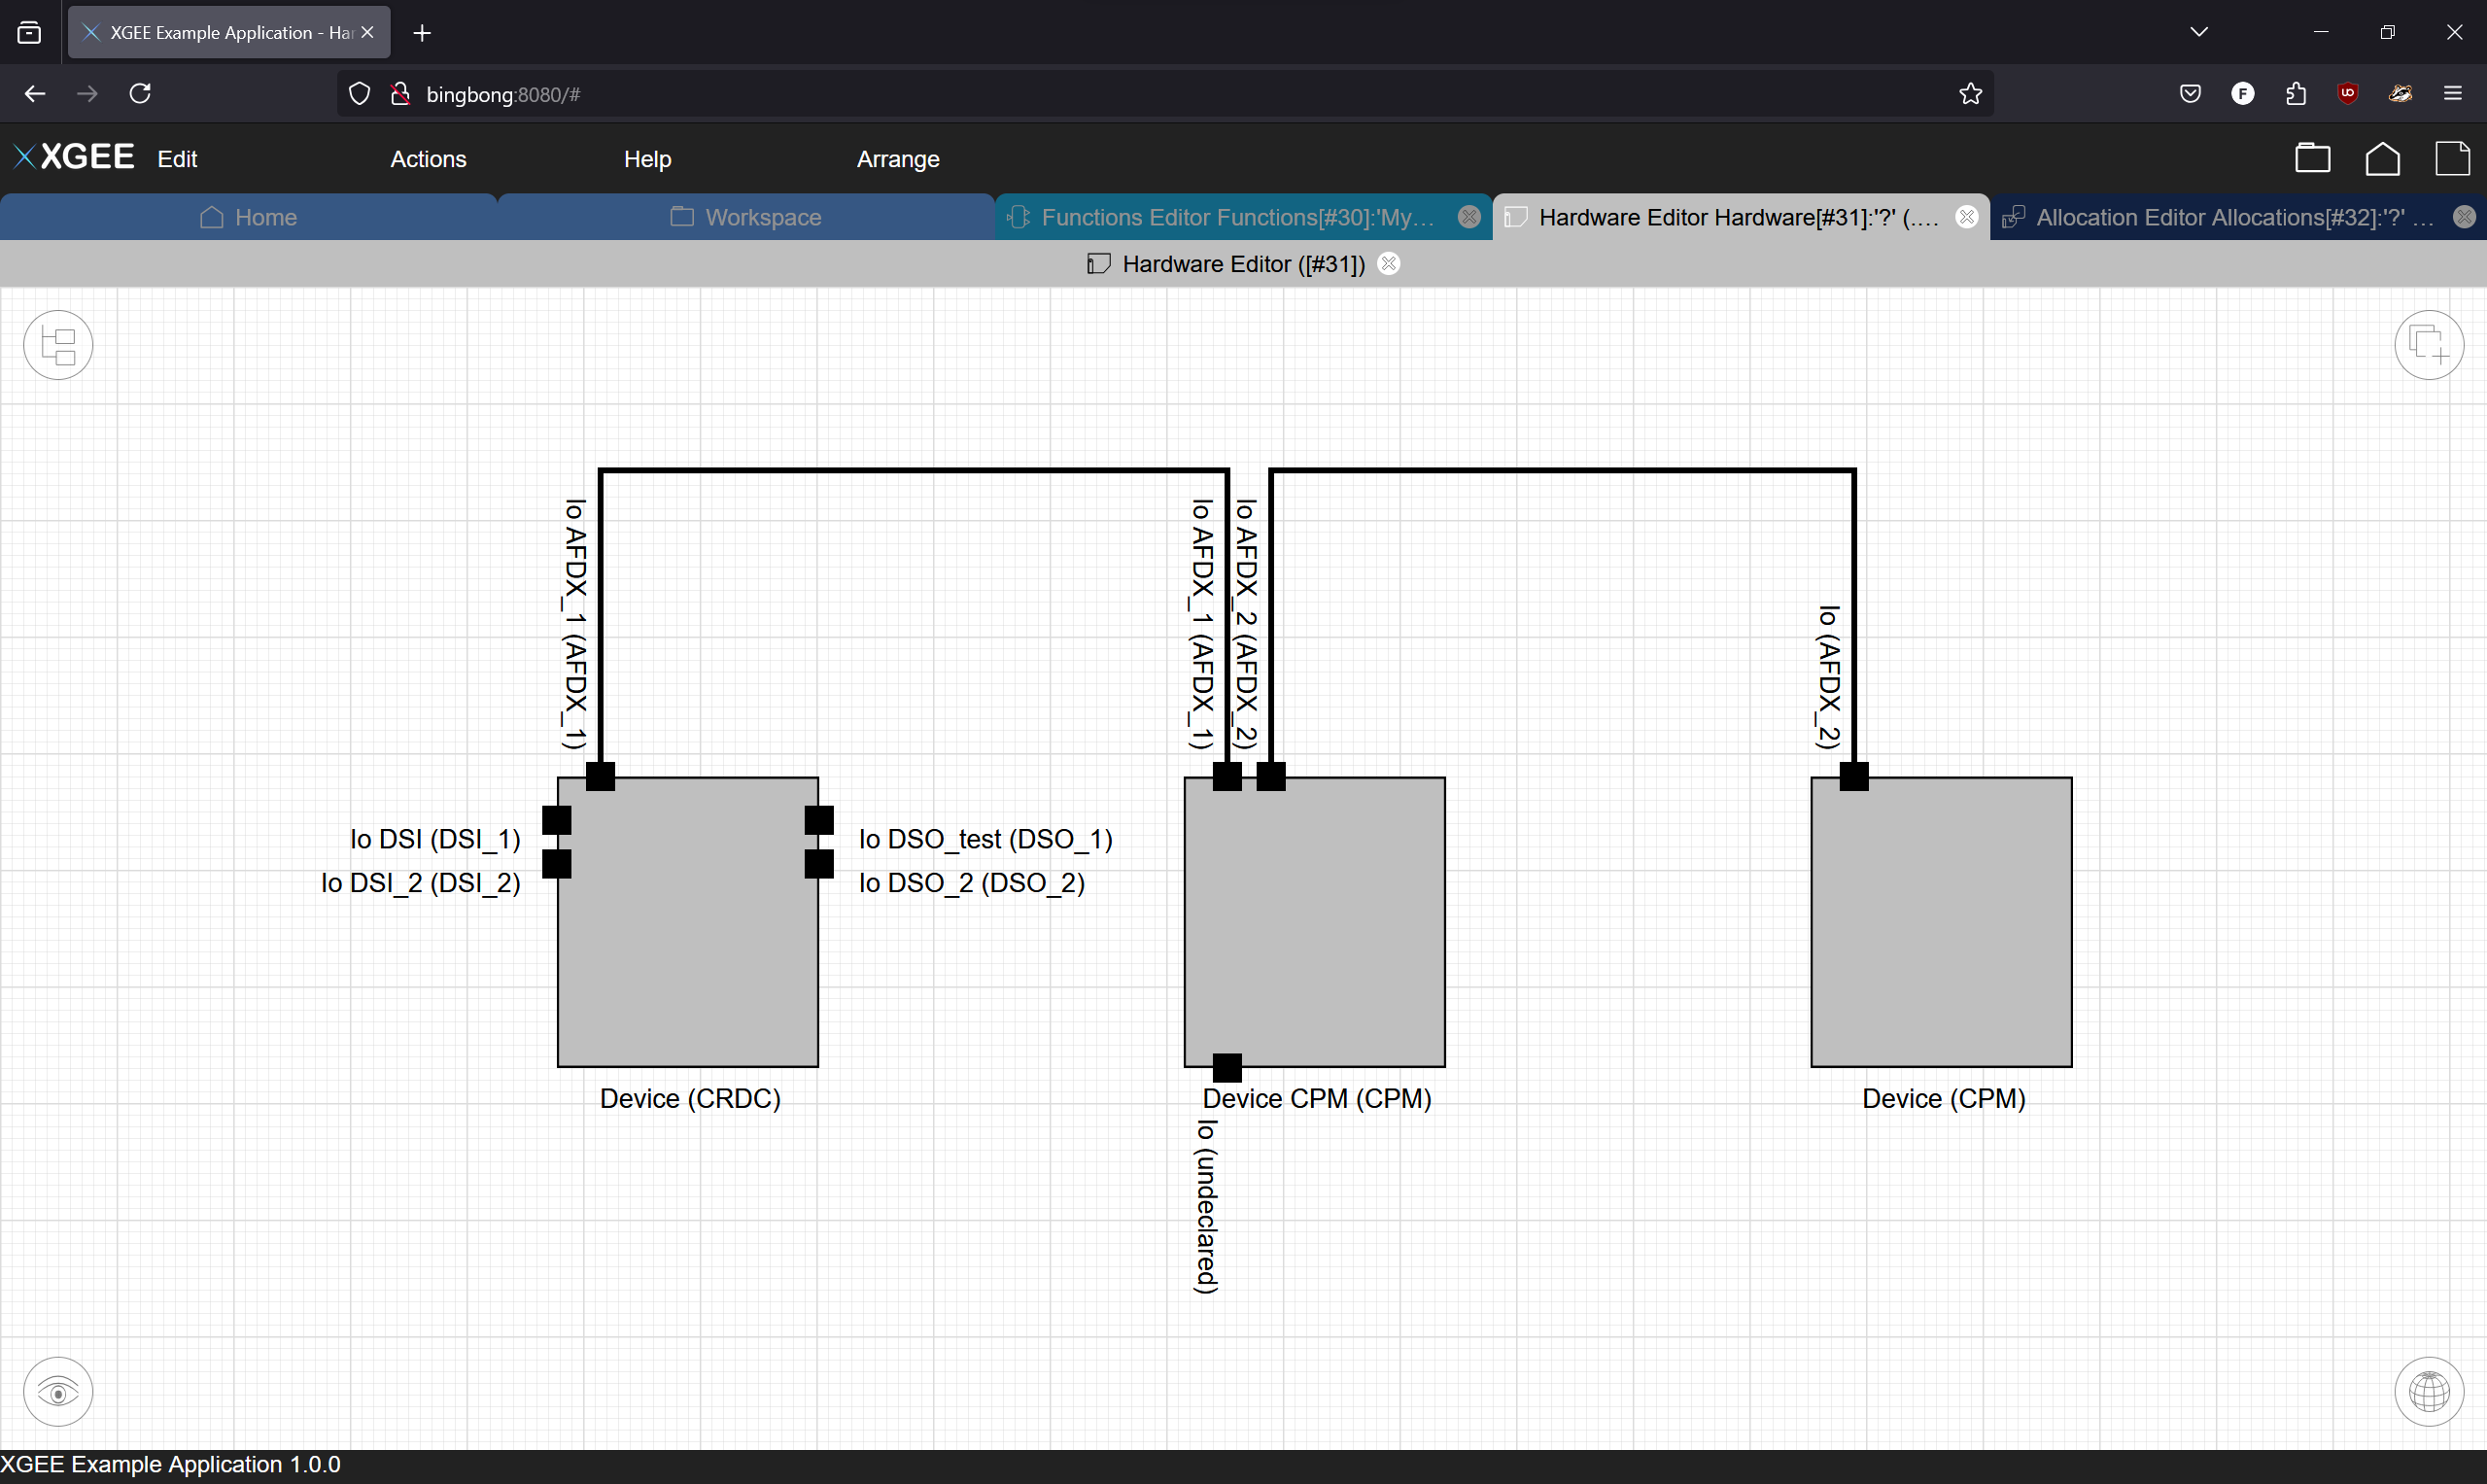
\includegraphics[width=\textwidth]{pictures/hardware_unaltered.png}
        \label{fig:hardware_unaltered}
    \end{minipage}
    \caption[Unaltered models as a basis for testcase generation]{Unaltered models as a basis for testcase generation.\\
    Left: Functions Layer, Right: Hardware Layer}
    \label{fig:unaltered_layers}
\end{figure}
The testcases enumerated in \autoref{tab:test_cases_text} only result in textual error indications. This is because the tested errors can not be detected during the tokenization or syntax steps of the verification pipeline, meaning that visually, the used tokens and their syntax are correct. The errors are only discovered during the comparison or instantiation steps, resulting in only a textual error indication. The first column of the table provides a zoomed-in view of a model containing the error. The second column provides a brief description of the testcase and the indicated textual errors.

\autoref{tab:functional_test_cases_no_errors} contains testcases without any simulated errors to illustrate the pipelines capability to deal with complex models including diverse vertices and intersecting connections. The first colummn provides a brief description, the second and third column provide the visualization within the functions layer and within the hardware layer of the \acrshort{xgee} editor.\\
While the tokenization is functional for three of \acrshort{xgee}s model layers, the allocations layer has not yet been implemented fully into the verification pipeline, meaning that there are currently no meaningful error indications when trying to verify a model in the allocations layer. Hence, the testcases are only shown for the functions and hardware layers.\\
A seperate testcase showcasing the capability of the tokenization pipeline of allocation models can be seen in \autoref{fig:allocations_found_tokens}. All found edges, bounding boxes and their respective token names are overlayed in green on the screenshot of the used model.
\newpage
\begin{longtable}{p{0.2\textwidth} >{\raggedright\arraybackslash}m{0.2\textwidth} >{\raggedright\arraybackslash}m{0.5\textwidth}}
    \caption{Results for test cases with textual and visual error indication.}
    \label{tab:test_cases}\\
    \toprule
    Test Case & Excerpt Visual Error Indication & Textual Error Indication \\
    \midrule
    \endfirsthead
    
    \multicolumn{3}{c}
    {{\bfseries Table \thetable\ continued from previous page}} \\
    \toprule
    Test Case & Excerpt Visual Error Indication & Textual Error Indication \\
    \midrule
    \endhead
    
    \midrule \multicolumn{3}{r}{{Continued on next page}} \\
    \endfoot
    
    \bottomrule
    \endlastfoot
    Functions Layer - Task too Small &  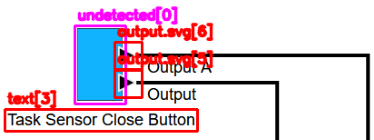
\includegraphics[width=1\linewidth]{pictures/20_task_too_small_output_clip.png} & \textbf{Tokenization}: untokenized pixels. \newline
        \textbf{Syntax}: ['text', 3] is missing a parent element. \newline
        \textbf{Syntax}: ['output.svg', 5] is missing a parent element. \newline
        \textbf{Syntax}: ['output.svg', 6] is missing a parent element. \newline
        \textbf{Instantiation}: output.svg[5] is not instantiated, association cannot connect. \newline
        \textbf{Comparison}: Task Sensor Close Button missing in recognized model. \newline
        \textbf{Comparison}: Signal Door System Logic: B $\rightarrow$ Actor Locked: A missing in recognized model. \newline
        \vdots \\
    \midrule
    Hardware Layer - Device too Small &  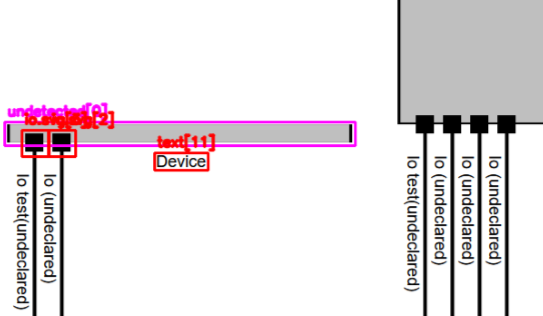
\includegraphics[width=1\linewidth]{pictures/21_device_too_small_output_clip.png} & \textbf{Tokenization}: untokenized pixels. \newline
        \textbf{Syntax}: ['text', 11] is missing a parent element. \newline
        \textbf{Syntax}: ['io.svg', 2] is missing a parent element. \newline
        \textbf{Syntax}: ['io.svg', 3] is missing a parent element. \\
    \midrule
    Functions Layer - Task Wrong Color &  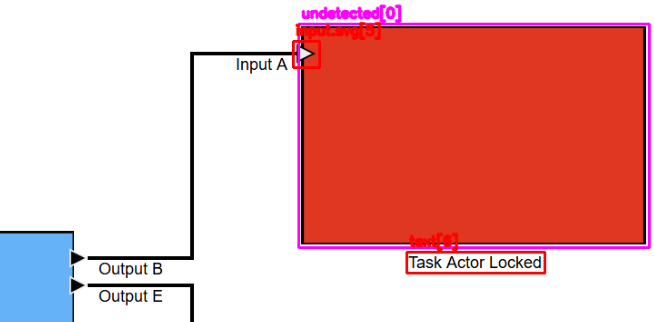
\includegraphics[width=1\linewidth]{pictures/31_wrong_color_task_output_clip.png} & \textbf{Tokenization}: untokenized pixels. \newline
        \textbf{Syntax}: ['text', 6] is missing a parent element. \newline
        \textbf{Syntax}: ['input.svg', 5] is missing a parent element. \newline
        \textbf{Instantiation}: input.svg[5] not instantiated, association cannot connect. \newline
        \textbf{Comparison}: Signal Door System Logic: B $\rightarrow$ Actor Locked: A missing in recognized model. \newline
        \textbf{Comparison}: Signal Door System Logic: E $\rightarrow$ System Logic Logging: 5 missing in recognized model. \newline
        \vdots \\
    \midrule
    Hardware Layer - Device Wrong Color &  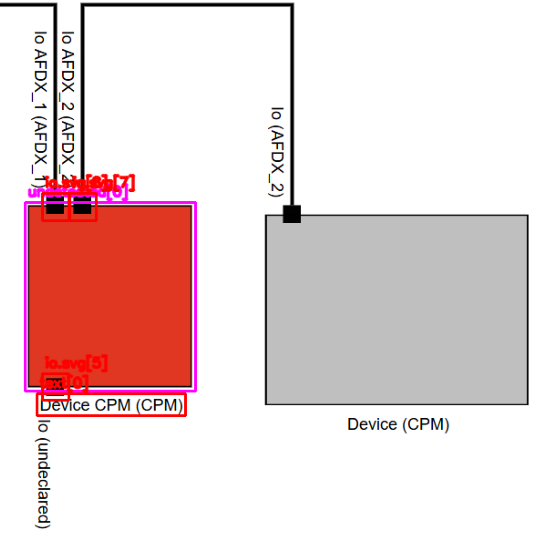
\includegraphics[width=1\linewidth]{pictures/32_wrong_color_task_output_clip.png} & \textbf{Tokenization}: untokenized pixels. \newline
        \textbf{Syntax}: ['text', 10] is missing a parent element. \newline
        \textbf{Syntax}: ['io.svg', 0] is missing a parent element. \newline
        \textbf{Syntax}: ['io.svg', 1] is missing a parent element. \newline
        \vdots \\
    \midrule
    Functions Layer - Free Floating Input & 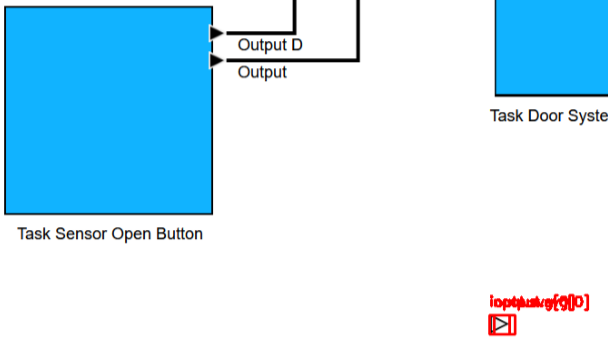
\includegraphics[width=1\linewidth]{pictures/40_free_floating_input_output_clip.png} & \textbf{Syntax}: ['input.svg', 0] is missing a parent element. \newline
        \textbf{Syntax}: ['output.svg', 1] is missing a parent element.\\
    \midrule
    Hardware Layer - Free Floating IO & 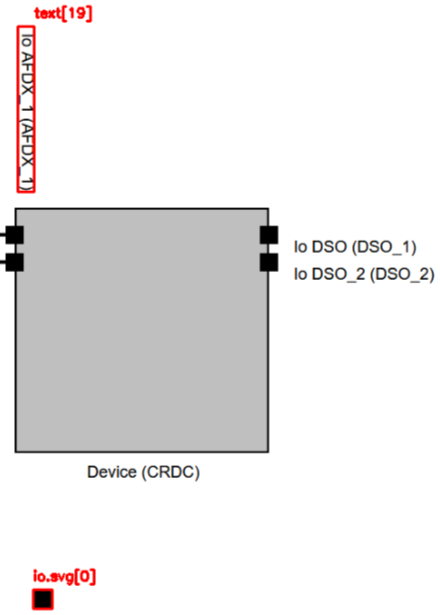
\includegraphics[width=1\linewidth]{pictures/41_free_floating_input_output_clip.png} & \textbf{Syntax}: ['text', 19] is missing a parent element. \newline
        \textbf{Syntax}: ['io.svg', 0] is missing a parent element. \\
    \midrule
    Functions Layer - Free Floating Star & 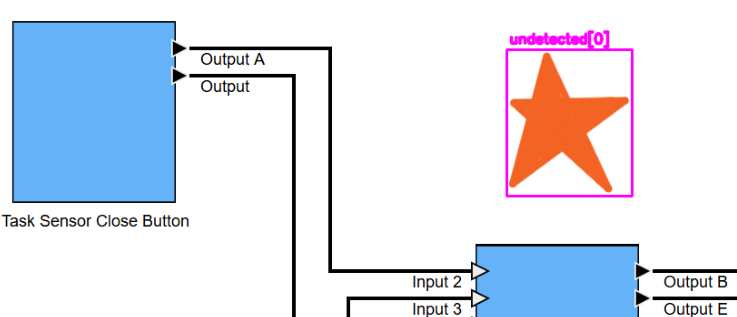
\includegraphics[width=1\linewidth]{pictures/42_free_floating_star_output_clip.png} & \textbf{Tokenization}: untokenized pixels. \\
    \midrule
    Hardware Layer - Free Floating Star & 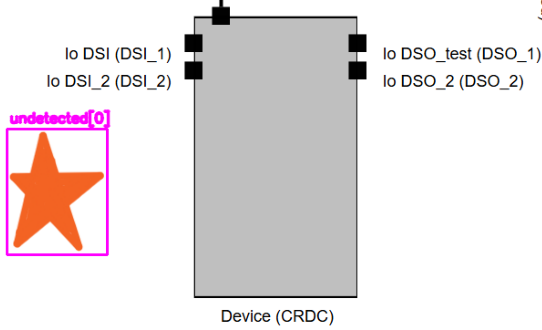
\includegraphics[width=1\linewidth]{pictures/43_free_floating_star_output_clip.png} & \textbf{Tokenization}: untokenized pixels. \\
    \midrule
    Functions Layer - Input Instead of Output & 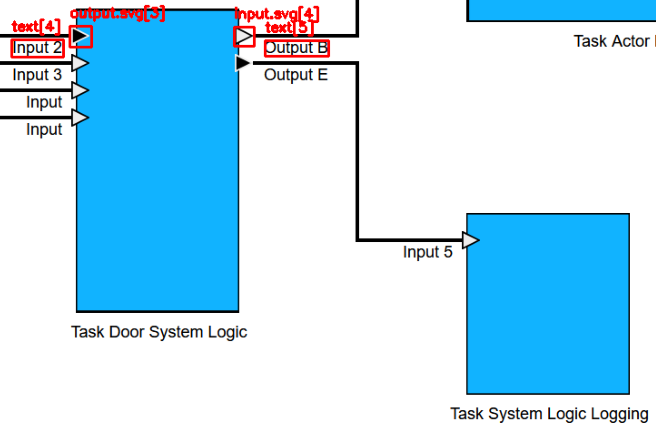
\includegraphics[width=1\linewidth]{pictures/50_input_instead_of_output_output_clip.png} & \textbf{Syntax}: ['text', 4] is missing a parent element. \newline
        \textbf{Syntax}: ['text', 4] is missing a parent element. \newline
        \textbf{Syntax}: ['input.svg', 4] is missing a parent element. \newline
        \textbf{Syntax}: ['output.svg', 3] is missing a parent element. \newline
        \textbf{Instantiation}: Failed to instantiate association. Endpoint input.svg. \newline
        \textbf{Instantiation}: Failed to instantiate association. Endpoint output.svg. \newline
        \textbf{Comparison}: Signal Door System Logic: B $\rightarrow$ Actor Locked: 1 missing. \newline
        \vdots \\
    \midrule
    Functions Layer - Signal Wrong Color & 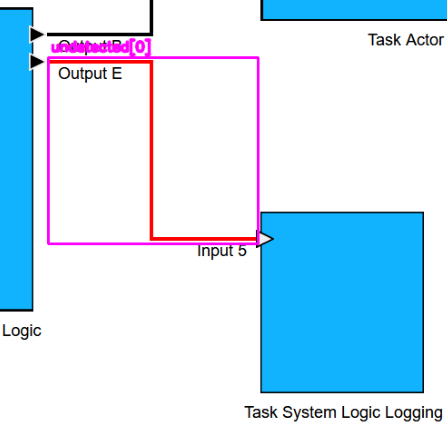
\includegraphics[width=1\linewidth]{pictures/32_signal_wrong_color_output_clip.png} & 
        \textbf{Tokenization}: untokenized pixels. \newline
        \textbf{Syntax}: ['text', 17] is missing a parent element. \newline
        \textbf{Comparison}: Number of Signals in the original model (6) does not match (5). \newline
        \textbf{Comparison}: Signal Door System Logic: E $\rightarrow$ System Logic Logging: 5 missing \\
    \midrule
    Hardware Layer - Signal Wrong Color & 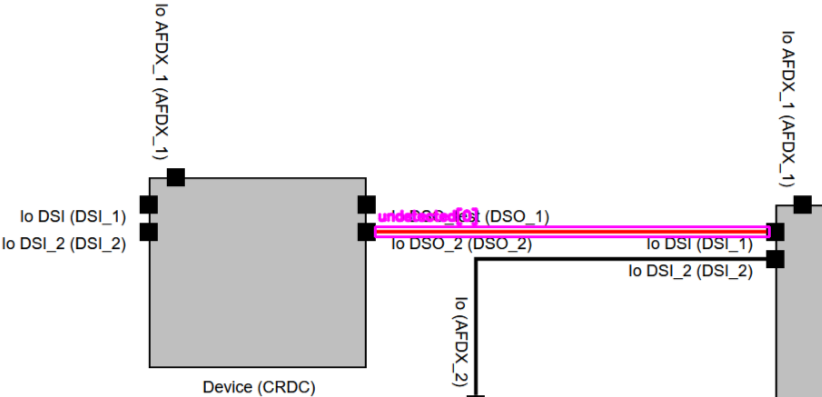
\includegraphics[width=1\linewidth]{pictures/33_signal_wrong_color_output_clip.png} & \textbf{Tokenization}: untokenized pixels. \\
    \midrule
    Functions Layer - Text too Far & 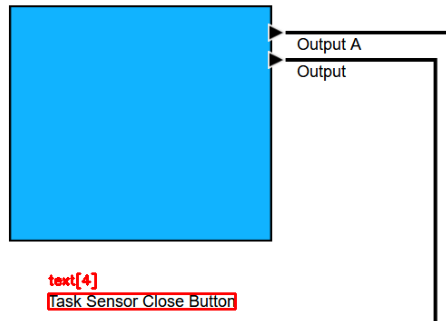
\includegraphics[width=\linewidth]{pictures/60_text_too_far_output_clip.png} & \textbf{Syntax}: ['text', 4] is missing a parent element. \newline
        \textbf{Comparison}: Task "Sensor Close Button" missing in recognized model. \newline
        \textbf{Comparison}: Signal Sensor Close Button: A $\rightarrow$ Door System \\
    \midrule
    Hardware Layer - Text too Near & 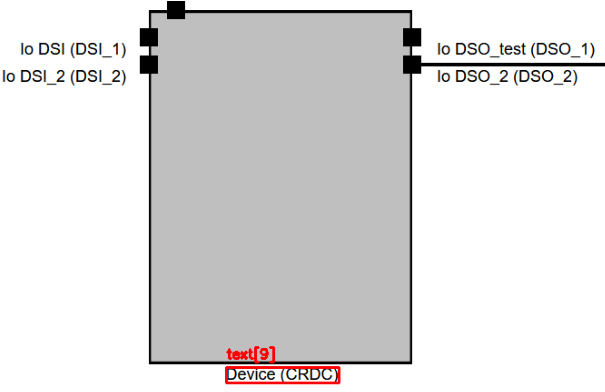
\includegraphics[width=1\linewidth]{pictures/61_text_too_far_output_clip.png} & \textbf{Syntax}:['text', 9] is missing a parent element. \\
\end{longtable}


\begin{longtable}{p{0.2\textwidth} >{\raggedright\arraybackslash}m{0.2\textwidth} >{\raggedright\arraybackslash}m{0.52\textwidth}}
    \caption{Results for test cases with textual error indication.}
    \label{tab:test_cases_text}\\
    \toprule
    Test Case & Excerpt Modified Screenshot & Textual Error Indication \\
    \midrule
    \endfirsthead
    
    \multicolumn{3}{c}{{\bfseries Table \thetable\ continued from previous page}} \\
    \toprule
    Test Case & Excerpt Modified Screenshot & Textual Error Indication \\
    \midrule
    \endhead
    
    \midrule \multicolumn{3}{r}{{Continued on next page}} \\
    \endfoot
    
    \bottomrule
    \endlastfoot
    
    New Task Hiding Other New Task & 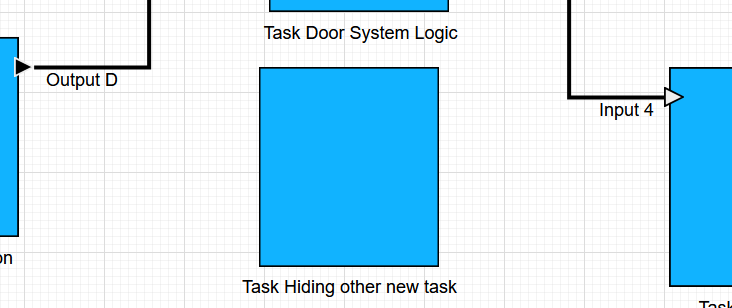
\includegraphics[width=\linewidth]{pictures/61_task_hides_task_input_clip.png} & \textbf{Comparison}: Task Hidden missing \\
    \midrule
    Task Out of Window & 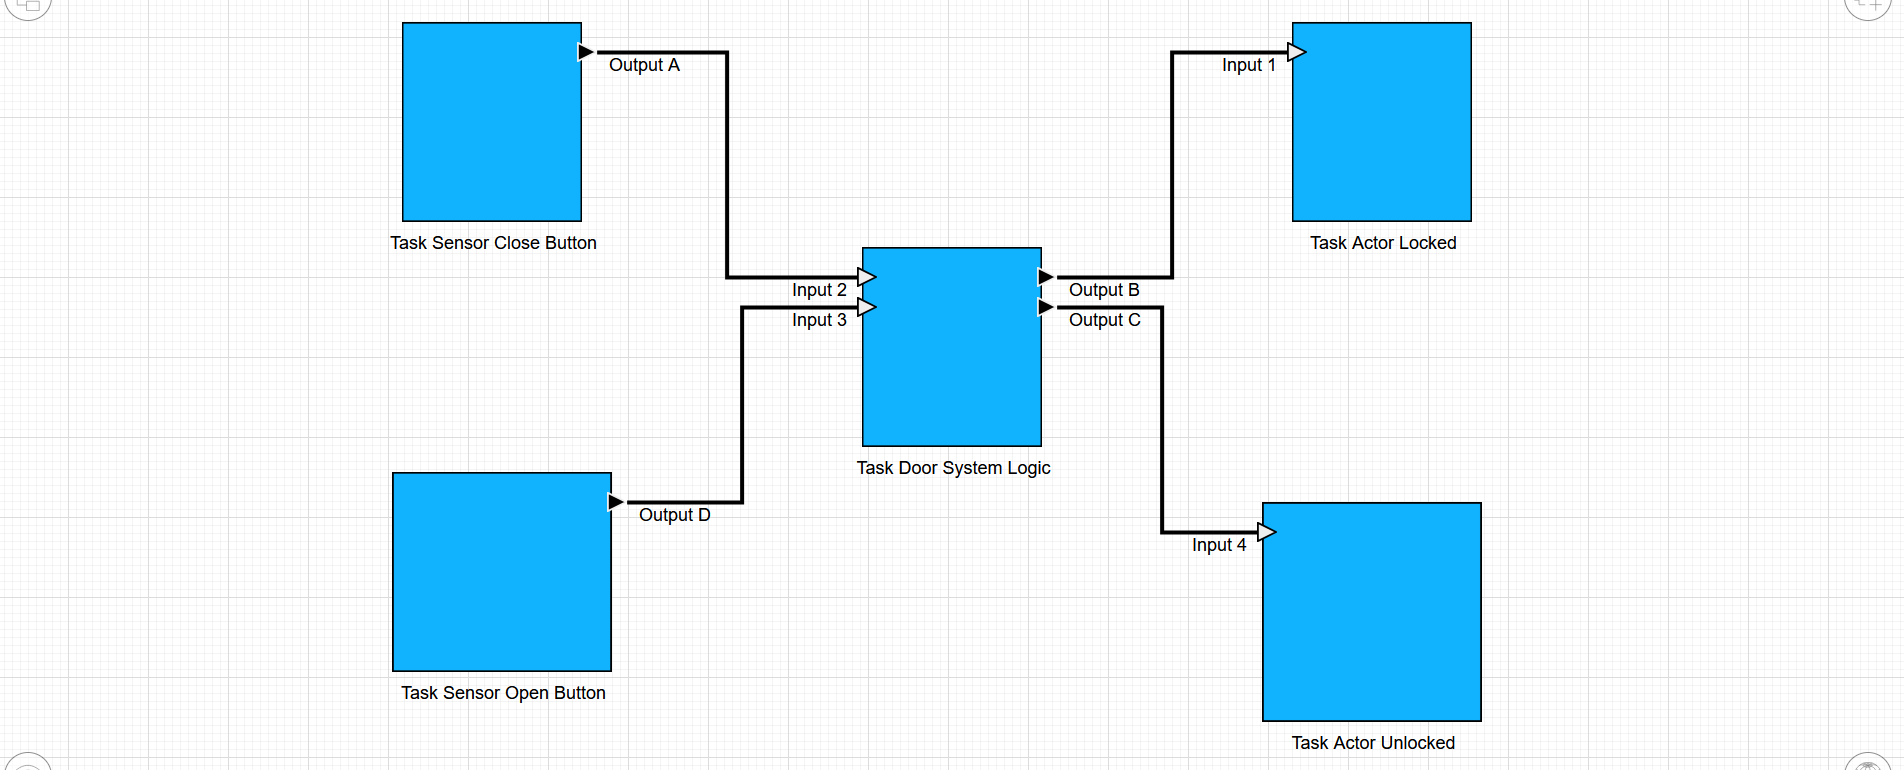
\includegraphics[width=\linewidth]{pictures/63_task_far_away_input_clip.png} & \textbf{Comparison}: Task Far Away missing \\
    \midrule
    Task Deleted in Editor, but Still in Model & 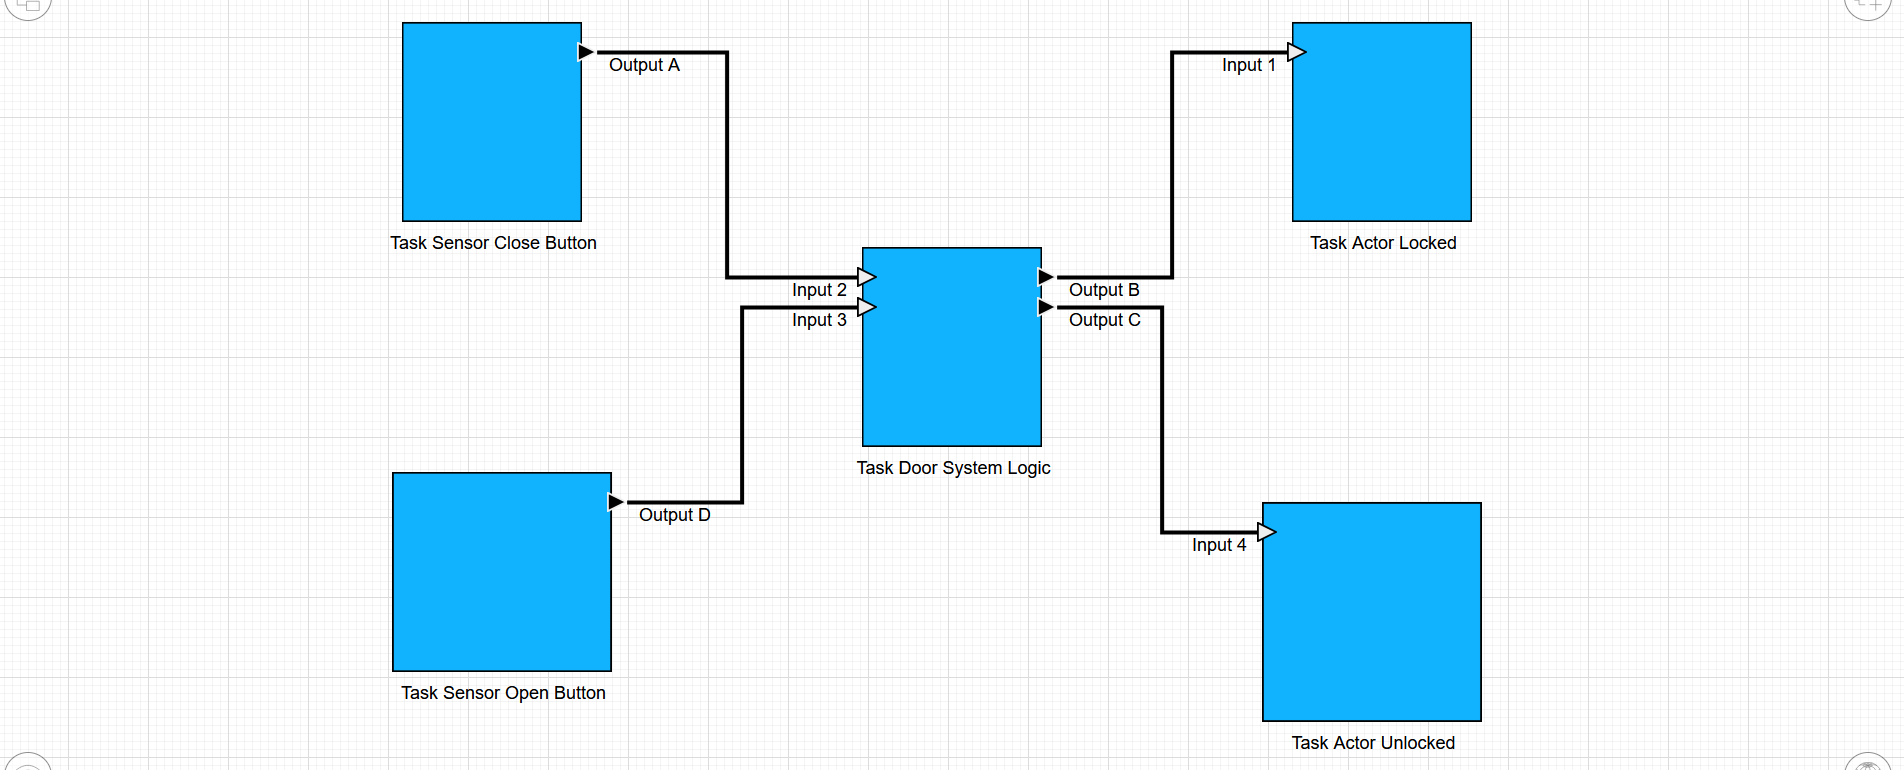
\includegraphics[width=\linewidth]{pictures/63_task_far_away_input_clip.png} & \textbf{Comparison}: Task New Task Already Deleted Missing \\
    \midrule
    Task Created, but Not Yet in Model & 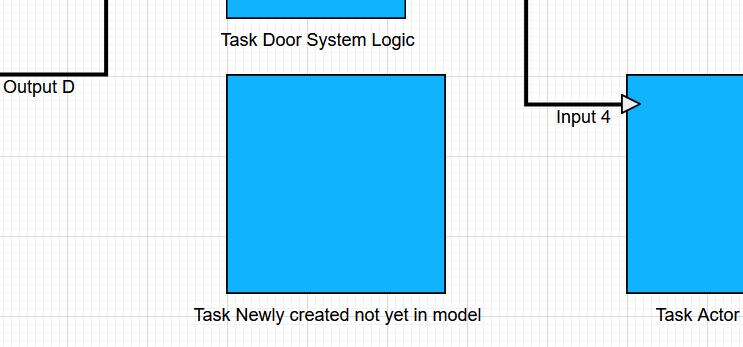
\includegraphics[width=\linewidth]{pictures/71_new_task_not_yet_in_model_input_clip.png} & \textbf{Comparison}: Task Newly Created Not Yet in Model Missing in Original Model \\
    \midrule
    Signal Not Connected to Input & 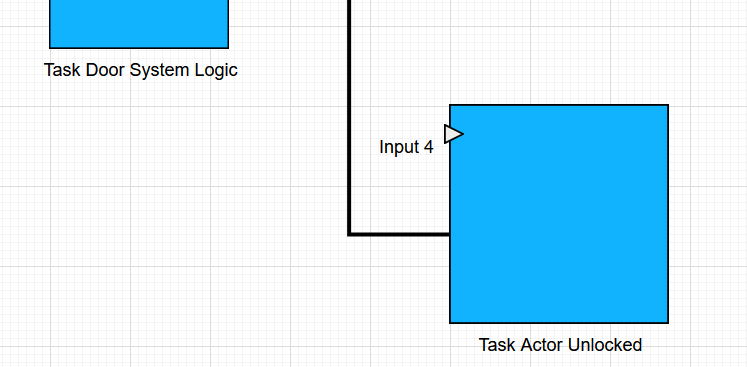
\includegraphics[width=\linewidth]{pictures/80_signal_not_connected_to_input_input_clip.png} & \textbf{Comparison}: Signal Door System Logic:C $\rightarrow$ Actor Unlocked:4 Missing \\
    \midrule
    Signal Connected to Wrong Port & 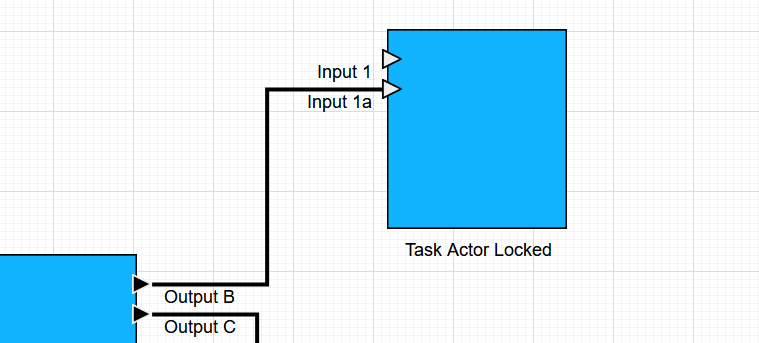
\includegraphics[width=\linewidth]{pictures/81_signal_wrong_port_correct_task_input_clip.png} & \textbf{Comparison}: Signal Door System Logic: B $\rightarrow$ Actor Locked: A Missing \newline \textbf{Comparison}: Signal Door System Logic: E $\rightarrow$ System Logic Logging: 5 Missing \\
    \midrule
    Overlapping Intersections & 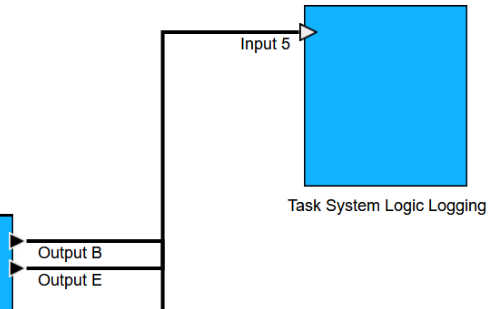
\includegraphics[width=\linewidth]{pictures/92_modified_task_name_input_clip.png} & \textbf{Comparison}: Sensor Open Button:D $\rightarrow$ Door System Logic:3 Missing \newline \textbf{Comparison}: Task Sensor Open Button Missing \\
    \midrule
    Changed Task Name, but Not Yet in Model & 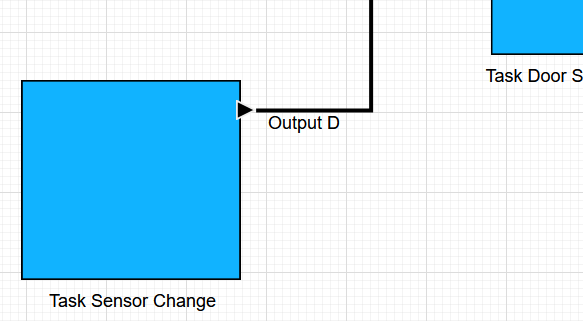
\includegraphics[width=\linewidth]{pictures/91_modified_task_name_input_clip.png} & \textbf{Comparison}: Sensor Open Button:D $\rightarrow$ Door System Logic:3 Missing \newline \textbf{Comparison}: Task Sensor Open Button Missing \\
    \midrule
    Encoding Error in Task Name & 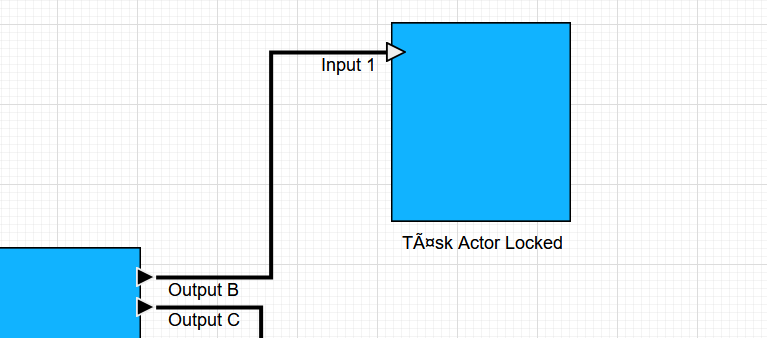
\includegraphics[width=\linewidth]{pictures/90_encoding_error_input_clip.png} & \textbf{Comparison}: Task Actor Locked Missing \newline \textbf{Comparison}: Signal Door System Logic:B $\rightarrow$ Actor Locked:1 Missing \\
\end{longtable}


\begin{table}[H]
    \caption{Functional Test Cases Demonstrating Correct System Behavior}
    \label{tab:functional_test_cases_no_errors}
    \begin{tabularx}{\textwidth}{@{}>{\hsize=.4\hsize\linewidth=\hsize}X m{0.3\textwidth} m{0.3\textwidth}@{}}
        \toprule
        Test case description & functions layer visualization & hardware layer visualization \\ 
        \midrule
        Processing of vertices with varying sizes and aspect ratios &  
        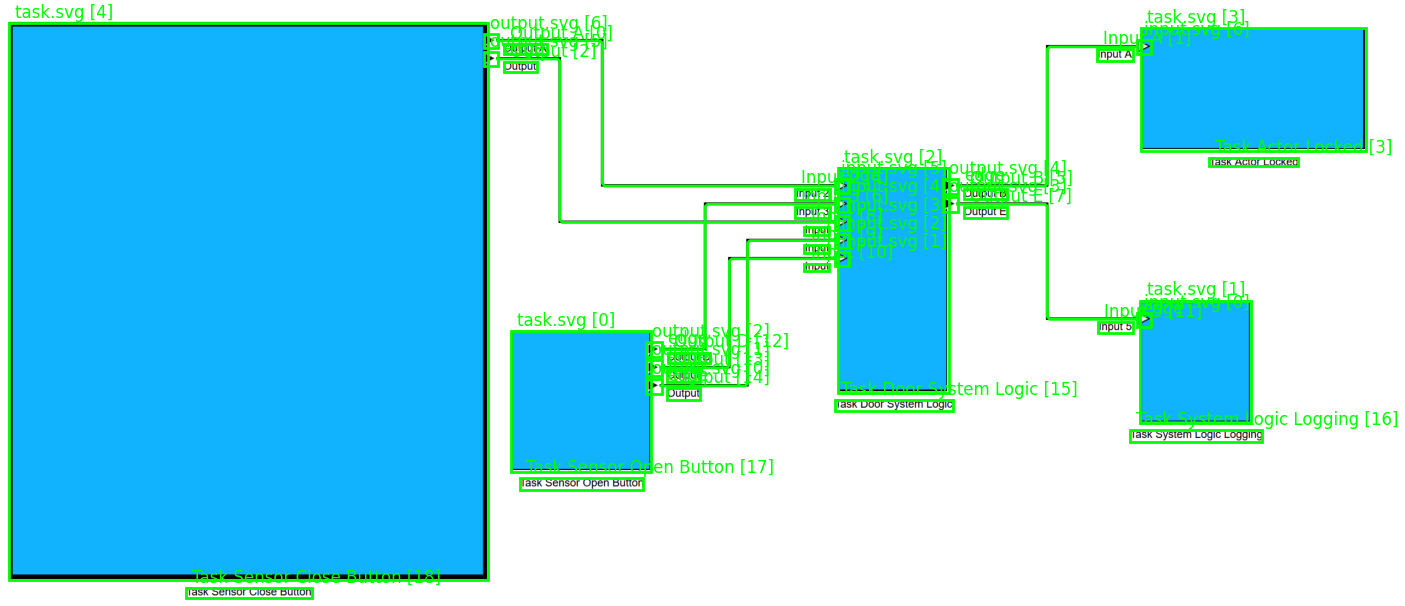
\includegraphics[width=\linewidth]{pictures/correct_task_size_input_clip.png} & 
        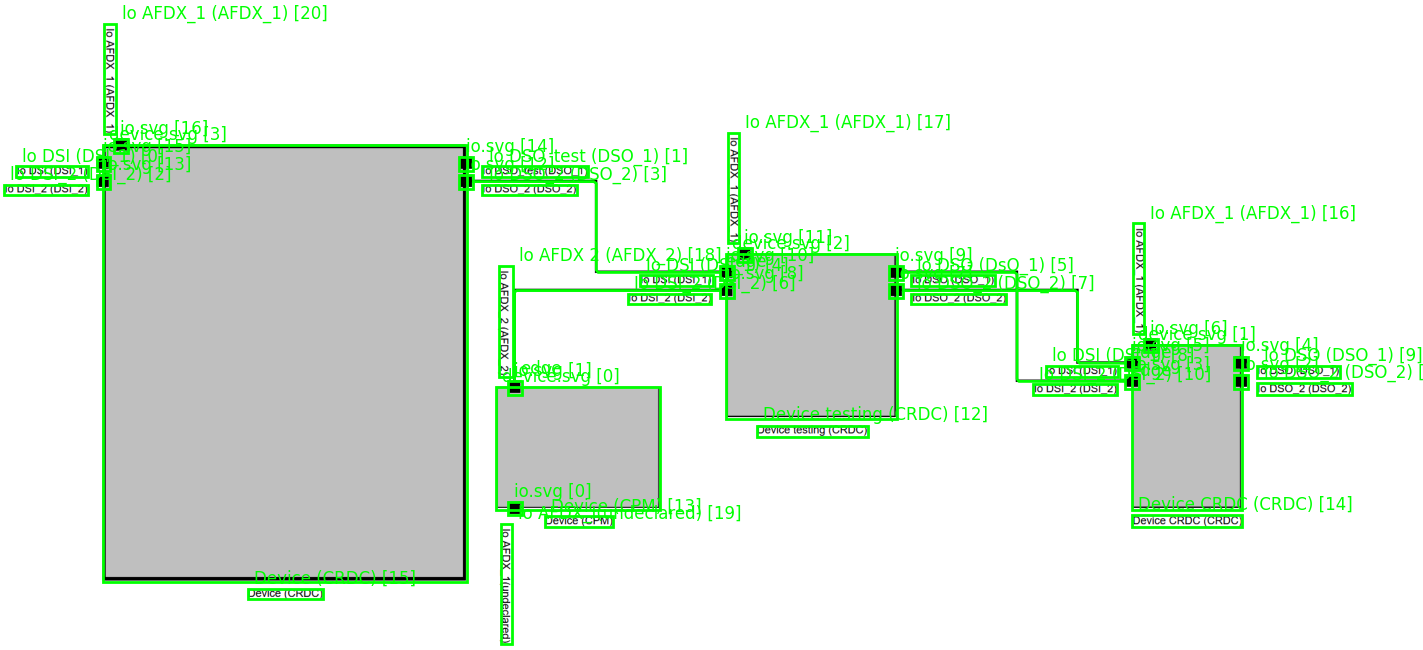
\includegraphics[width=\linewidth]{pictures/correct_task_size_output_clip.png} \\

        \midrule
        Recognition of complex signal intersections in close proximity &  
        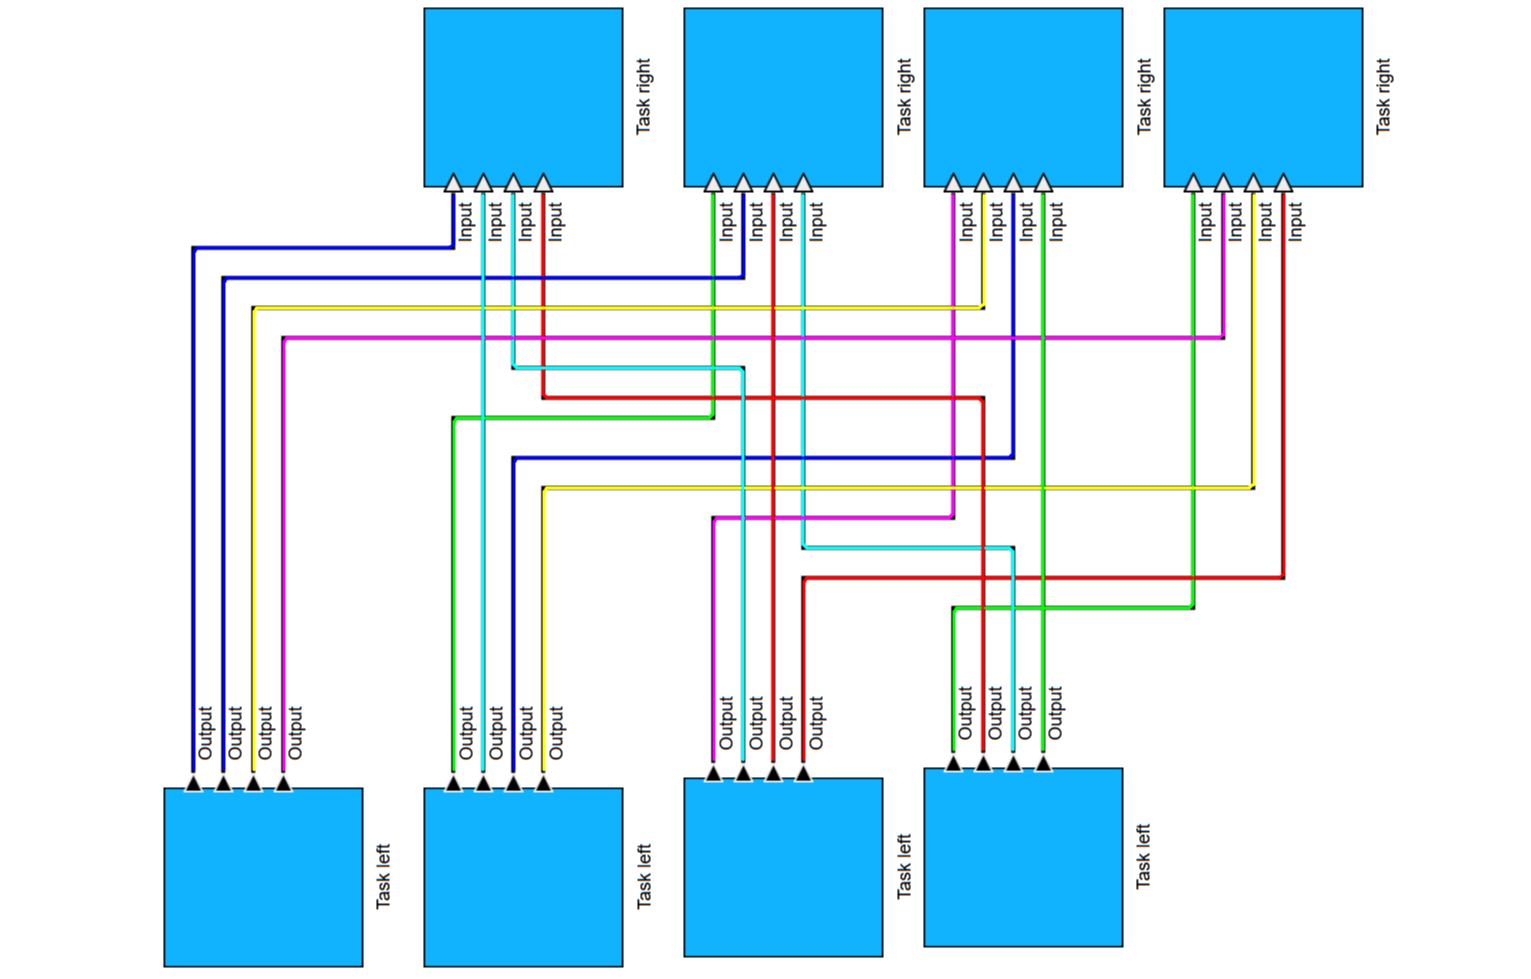
\includegraphics[width=\linewidth]{pictures/many_intersections.png} & 
        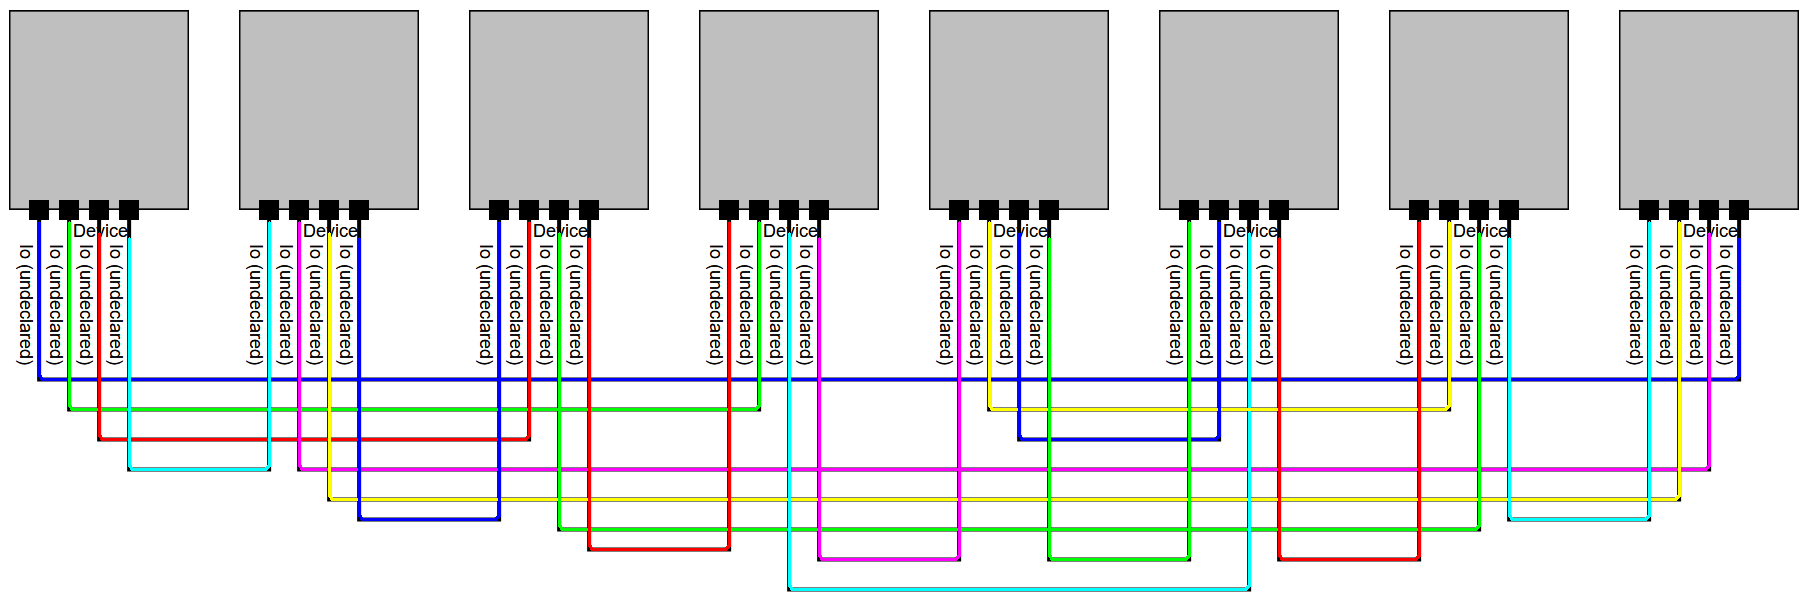
\includegraphics[width=\linewidth]{pictures/many_intersections_hardware.png} \\

        \midrule
        Function / device has the wrong color - but is still detected by the template matching method. &  
        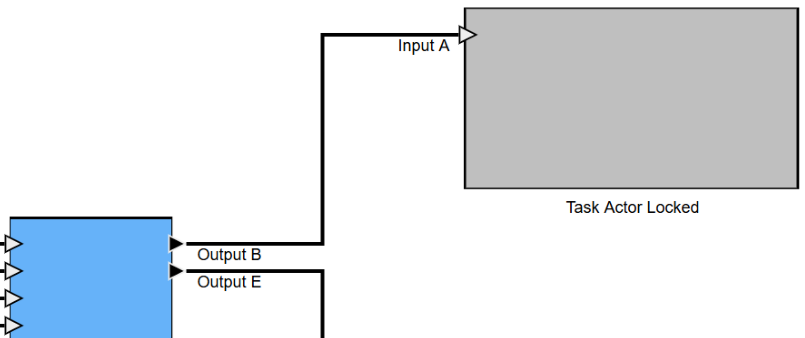
\includegraphics[width=\linewidth]{pictures/one_in_grey_input_clip.png} & 
        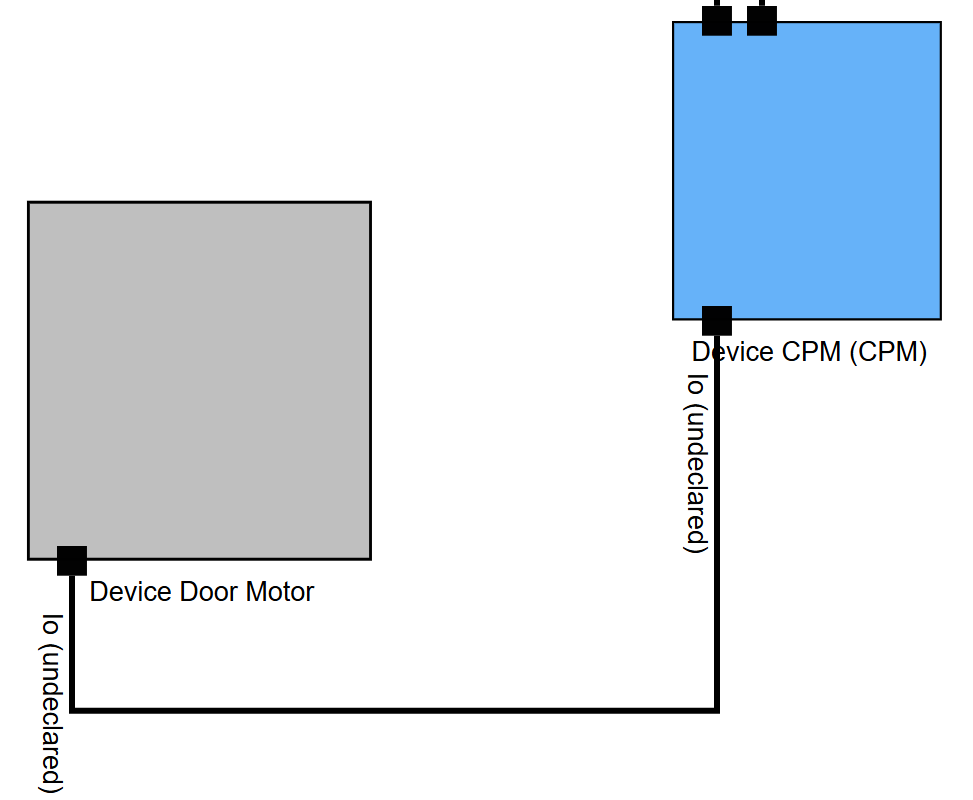
\includegraphics[width=\linewidth]{pictures/one_in_blue_input_clip.png} \\
        \bottomrule
    \end{tabularx}
\end{table}